\documentclass{beamer}
\usetheme{Darmstadt}
\usepackage{graphicx}
\usepackage[style=authortitle-ibid,backend=biber]{biblatex}
\addbibresource{refs.bib}
\graphicspath{ {images/} }

\title{Pothole Reconnaissance Network}
\subtitle{Tech for Good}
\author[Smith, Tsaris, Turnbull, Waldock]{H.~Smith \and A.~Tsaris \and L.~Turnbull \and L.~Waldock}
\institute[5J]{Group 5J}
\date{\today}

\AtBeginSection[]
{
  \begin{frame}
    \frametitle{Table of Contents}
    \tableofcontents[currentsection]
  \end{frame}
}

\begin{document}


\frame{\titlepage}

\section{The Problem}

\begin{frame}{What is a pothole?}

\begin{columns}

\column{0.6\linewidth}

How potholes develop:
\begin{enumerate}
    \item Cracks in the road develop from wear-and-tear by vehicles.
    \item Water seeps into these cracks.
    \item The water freezes, expanding the cracks --- the pothole is formed.\footnote[frame]{\cite{how-are-potholes-formed}}
\end{enumerate}
Potholes in the road are a challenge and a danger to many drivers and cyclists.

\column{0.4\linewidth}
\begin{figure}
    \includegraphics[width=3.5cm]{potholes}
    \caption{Picture of a pothole\footnote[frame]{\cite{pothole-pic}}}
\end{figure}

\end{columns}

\end{frame}

\begin{frame}{Health Risks}

They pose a risk to \alert{health} as:

\begin{itemize}
    \item Cars can lose control after driving into them, potentially crashing into other cars, cyclists and pedestrians.
    \item Drivers may attempt to swerve around them when it is unsafe to do so.
    \begin{itemize}
        \item For example, driving close to parked cars, abruptly driving into another lane, etc.
    \end{itemize}
    \item Cyclists can crash into them, potentially flipping-over and injuring themselves.
\end{itemize}

\end{frame}

\begin{frame}{Financial Risks}

    They also pose a \alert{financial} risk due to the cost of vehicle repair.

    \begin{itemize}
        \item Cars are often damaged after driving over potholes.
        \begin{itemize}
            \item cracks on windscreen
            \item burst tyres
            \item damage to suspension
            \item and more…
        \end{itemize}
        \item Drivers called out the RAC to 5,153 breakdowns caused by potholes in Q4 2023 \footcite{car-breakdowns}.
    \end{itemize}

\end{frame}

\begin{frame}{Why Solve This Issue?}
    \begin{itemize}
        \item Until we use indestructible road material, potholes will always be an issue --- and so will these risks.
        \item However, we can take steps to \emph{mitigate} this by filling potholes as often and promptly as possible.
        \item A complimentary system can be created to alert local councils of the location of potholes, so that they can be repaired swiftly.
    \end{itemize}

    \begin{block}{From the BSC Code of Conduct:}
    ``[You shall] have due regard for public health, privacy, security and wellbeing of others and
    the environment''\footnote[frame]{\cite{bcs-coc}}
    \end{block}
\end{frame}

\section{The Current Solution}

\begin{frame}{Reporting a Pothole}
    Potholes can currently be reported online through government websites.
\end{frame}

\begin{frame}
    Users can access \url{https://www.gov.uk/report-pothole}, and enter the postcode for the pothole found.
    \begin{figure}
        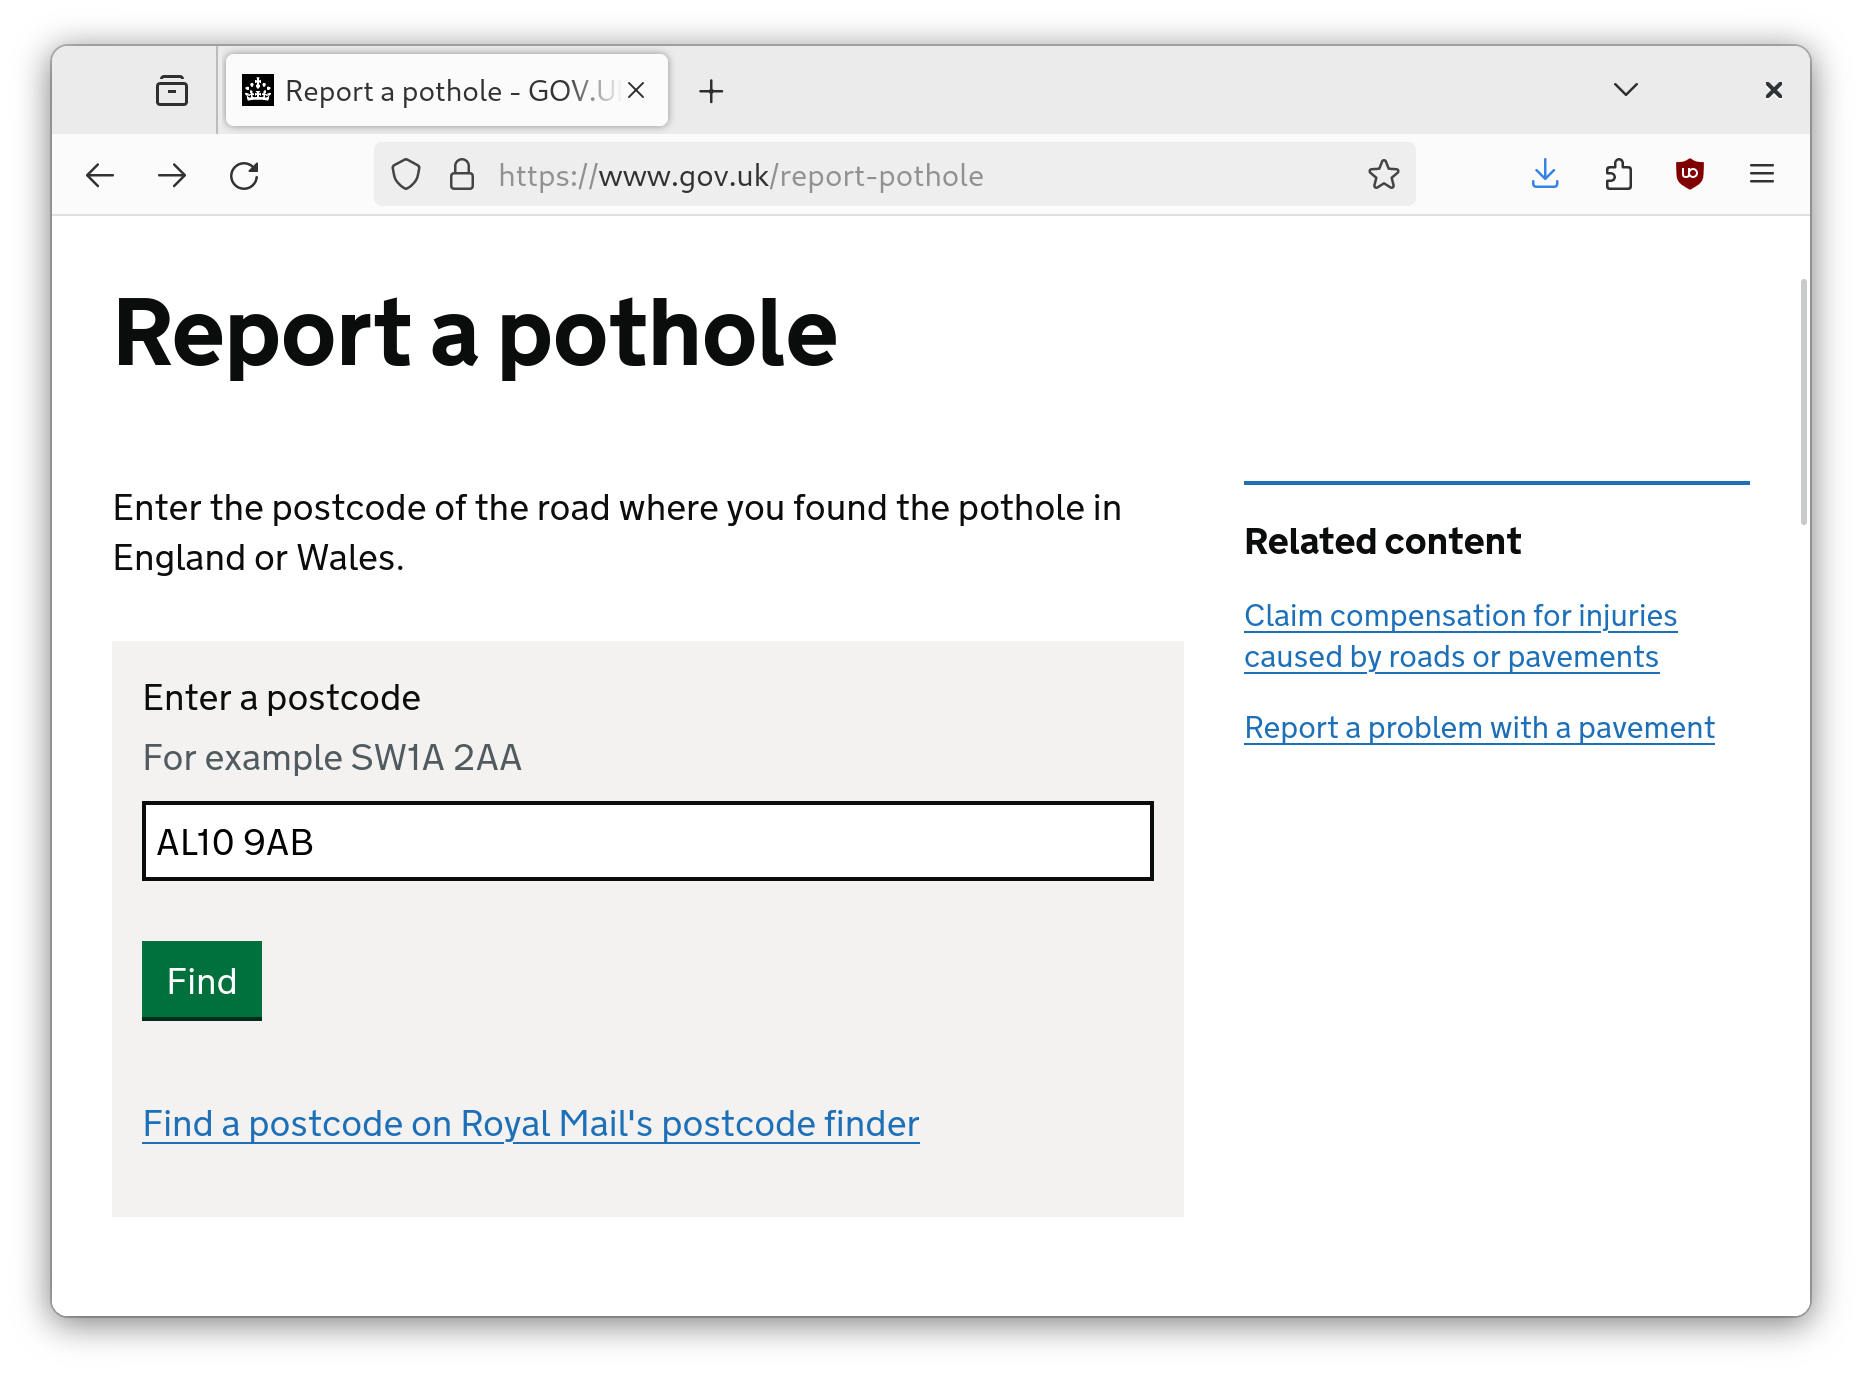
\includegraphics[width=8.3cm]{gov-uk.png}
        \caption{A screenshot of GOV.UK's site to report a pothole}
    \end{figure}
\end{frame}

\begin{frame}
    They are then redirected to their local council's site.
    \begin{figure}
        \includegraphics[width=8.3cm]{hertfordshire-report.png}
        \caption{A screenshot of Hertfordshire County Council's page to report a pothole}
    \end{figure}
\end{frame}

\begin{frame}{Problems With This}
    Motorists cannot report potholes in real time.
    \begin{itemize}
        \item It would be unsafe and illegal to use these websites \emph{while driving} \footcite{highway-code}.
        \item Therefore, users must wait until they safely park before they can submit a report.
    \end{itemize}
\end{frame}

\begin{frame}{Problems With This}
    By the time users can safely access the website(s):
    \begin{itemize}
        \item They may have forgotten about the pothole, and likely won't report it.
        \item Or they may remember the pothole, but cannot recall its exact location (needed in the report).
        \item Or they may not simply have the time or patience to manually submit a report for every pothole they find on the road.
    \end{itemize}
\end{frame}

\begin{frame}[allowframebreaks]{References}
    \printbibliography
\end{frame}

\end{document}